%%%%%%%%%%%%%%%%%%%%%%%%%%%%%%%%%%%%%%%%%%%%%%%%%%%%%%%%%%%%%%%%%%%%%
%                                                                   %
%	CHAPTER SIX: COMMUNICATION WALL: GRAPH500                       %
%                                                                   %
%%%%%%%%%%%%%%%%%%%%%%%%%%%%%%%%%%%%%%%%%%%%%%%%%%%%%%%%%%%%%%%%%%%%%

\chapter{Communication Wall: Graph500} 

\section{Introduction}
In order to face the communication wall in our metric for accelerators, we choose the Graph500 problem. 
This benchmark is based on huge tree traversal through a randomly generated graph. 
We already work on this kind of example with the first implementation of the Langford algorithm.
The Graph500 push this example to its limits using terabyte to petabytes of data to represent the graph on which the traversal is executed. 
In this case the computation is absent or just reduce to tests on datum.
This metric targets directly the memory and communication wall in irregular case. 

In this part we present the benchmark itself, from the graph generation to the traversal. 
We focus on the BFS part, we do not work on the latest Graph500 using SSSP. 
We explain why this benchmark is perfect to target communication wall and memory wall. 
We present our implementation on GPUs and the results compared to the multi-core processor version.

\subsection{Breadth First Search}
The most commonly used search algorithms for graphs are Breadth First Search (BFS) and Depth First Search (DFS).
Many graph analysis methods, such as the finding of shortest path for unweighted graphs and centrality, are based on BFS. 

As it is a standard approach method in graph theory, its implementation and optimization require extensive work. 
This algorithm can be seen as frontier expansion and exploration. 
At each step the frontier is expanded with the unvisited neighbors.  

\begin{algorithm}

\begin{algorithmic}[1]
\Function{compute\_BFS}{$G=(V,E)$:~graph representation, $v_s$:~source vertex, $In$:~current level input, $Out$:~current level output, $Vis$: already visited vertices}
\State $In \gets \{v_s\}$;
\State $Vis \gets \{v_s\}$;
\State $P(v) \gets \perp \forall v \in V$;
\While{$In \neq \emptyset$}
	\State $Out \gets \emptyset$
	\For{$u \in In$}
		\For{$v | (u,v) \in E$}
			\If{$v \notin Vis$}
				\State $Out \leftarrow Out \cup \{v\}$;
				\State $Vis \gets Vis \cup \{v\}$;
				\State $P(v) \leftarrow u$;
			\EndIf
		\EndFor
	\EndFor
	\State $In \gets Out$
\EndWhile
\EndFunction
\end{algorithmic}
\caption{Sequential Breadth First Search algorithm}
\label{alg:bfs_squential}
\end{algorithm}

The sequential and basic algorithm is well known and is presented on Algorithm~\ref{alg:bfs_squential}.

\begin{figure}
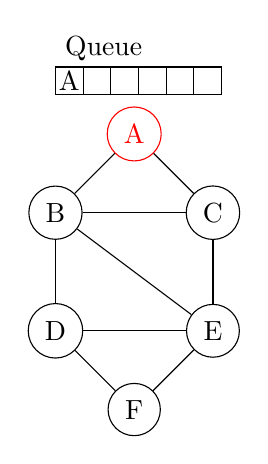
\begin{tikzpicture}
	\node [draw,circle,red] (node A) at (1,3.5) {A};
	\node [draw,circle] (node B) at (0,2.5) {B};
	\node [draw,circle] (node C) at (2,2.5) {C};
	\node [draw,circle] (node D) at (0,1) {D};
	\node [draw,circle] (node E) at (2,1) {E};
	\node [draw,circle] (node F) at (1,0) {F};
	
	\draw (node A) -- (node B);
	\draw (node A) -- (node C);
	\draw (node B) -- (node D);
	\draw (node B) -- (node E);
	\draw (node C) -- (node E);
	\draw (node D) -- (node F);
	\draw (node E) -- (node F);
	\draw (node B) -- (node C);
	\draw (node D) -- (node E);

	% The array under the graph
	%\foreach \x in{0,...,5}{\draw (\x*1em,-1) rectangle (\x*1em+1em,-1+1em);}
	\draw (0,4) rectangle (1em,4.35) node[pos=.5] {A};
	\draw (1em,4) rectangle (2em,4.35);
	\draw (2em,4) rectangle (3em,4.35);
	\draw (3em,4) rectangle (4em,4.35);
	\draw (4em,4) rectangle (5em,4.35);
	\draw (5em,4) rectangle (6em,4.35);

	\node [anchor=south west] at (0,4.3) {Queue};
\end{tikzpicture}
\hfill
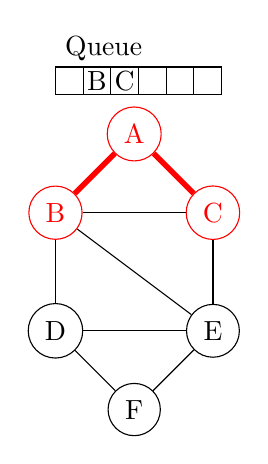
\begin{tikzpicture}
	\node [draw,circle,red] (node A) at (1,3.5) {A};
	\node [draw,circle,red] (node B) at (0,2.5) {B};
	\node [draw,circle,red] (node C) at (2,2.5) {C};
	\node [draw,circle] (node D) at (0,1) {D};
	\node [draw,circle] (node E) at (2,1) {E};
	\node [draw,circle] (node F) at (1,0) {F};
	
	\draw [red,line width=2pt] (node A) -- (node B);
	\draw [red,line width=2pt] (node A) -- (node C);
	\draw (node B) -- (node D);
	\draw (node B) -- (node E);
	\draw (node C) -- (node E);
	\draw (node D) -- (node F);
	\draw (node E) -- (node F);
	\draw (node B) -- (node C);
	\draw (node D) -- (node E);

	% The array under the graph
	%\foreach \x in{0,...,5}{\draw (\x*1em,-1) rectangle (\x*1em+1em,-1+1em);}
	\draw (0,4) rectangle (1em,4.35) node[pos=.5] {};
	\draw (1em,4) rectangle (2em,4.35) node[pos=.5] {B};
	\draw (2em,4) rectangle (3em,4.35) node[pos=.5] {C};
	\draw (3em,4) rectangle (4em,4.35) node[pos=.5] {};
	\draw (4em,4) rectangle (5em,4.35) node[pos=.5] {};
	\draw (5em,4) rectangle (6em,4.35) node[pos=.5] {};

	\node [anchor=south west] at (0,4.3) {Queue};
\end{tikzpicture}
\hfill
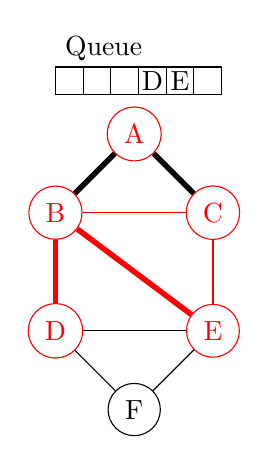
\begin{tikzpicture}
	\node [draw,circle,red] (node A) at (1,3.5) {A};
	\node [draw,circle,red] (node B) at (0,2.5) {B};
	\node [draw,circle,red] (node C) at (2,2.5) {C};
	\node [draw,circle,red] (node D) at (0,1) {D};
	\node [draw,circle,red] (node E) at (2,1) {E};
	\node [draw,circle] (node F) at (1,0) {F};
	
	\draw [line width=2pt] (node A) -- (node B);
	\draw [line width=2pt] (node A) -- (node C);
	\draw [red,line width=2pt] (node B) -- (node D);
	\draw [red,line width=2pt] (node B) -- (node E);
	\draw [red] (node C) -- (node E);
	\draw (node D) -- (node F);
	\draw (node E) -- (node F);
	\draw [red] (node B) -- (node C);
	\draw (node D) -- (node E);

	% The array under the graph
	%\foreach \x in{0,...,5}{\draw (\x*1em,-1) rectangle (\x*1em+1em,-1+1em);}
	\draw (0,4) rectangle (1em,4.35) node[pos=.5] {};
	\draw (1em,4) rectangle (2em,4.35) node[pos=.5] {};
	\draw (2em,4) rectangle (3em,4.35) node[pos=.5] {};
	\draw (3em,4) rectangle (4em,4.35) node[pos=.5] {D};
	\draw (4em,4) rectangle (5em,4.35) node[pos=.5] {E};
	\draw (5em,4) rectangle (6em,4.35) node[pos=.5] {};

	\node [anchor=south west] at (0,4.3) {Queue};
\end{tikzpicture}
\hfill
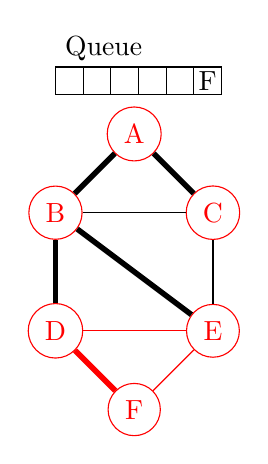
\begin{tikzpicture}
	\node [draw,circle,red] (node A) at (1,3.5) {A};
	\node [draw,circle,red] (node B) at (0,2.5) {B};
	\node [draw,circle,red] (node C) at (2,2.5) {C};
	\node [draw,circle,red] (node D) at (0,1) {D};
	\node [draw,circle,red] (node E) at (2,1) {E};
	\node [draw,circle,red] (node F) at (1,0) {F};
	
	\draw [line width=2pt] (node A) -- (node B);
	\draw [line width=2pt] (node A) -- (node C);
	\draw [line width=2pt]  (node B) -- (node D);
	\draw [line width=2pt] (node B) -- (node E);
	\draw (node C) -- (node E);
	\draw [red,line width=2pt] (node D) -- (node F);
	\draw [red] (node E) -- (node F);
	\draw (node B) -- (node C);
	\draw [red] (node D) -- (node E);

	% The array under the graph
	%\foreach \x in{0,...,5}{\draw (\x*1em,-1) rectangle (\x*1em+1em,-1+1em);}
	\draw (0,4) rectangle (1em,4.35) node[pos=.5] {};
	\draw (1em,4) rectangle (2em,4.35) node[pos=.5] {};
	\draw (2em,4) rectangle (3em,4.35) node[pos=.5] {};
	\draw (3em,4) rectangle (4em,4.35) node[pos=.5] {};
	\draw (4em,4) rectangle (5em,4.35) node[pos=.5] {};
	\draw (5em,4) rectangle (6em,4.35) node[pos=.5] {F};

	\node [anchor=south west] at (0,4.3) {Queue};
\end{tikzpicture}
\hfill
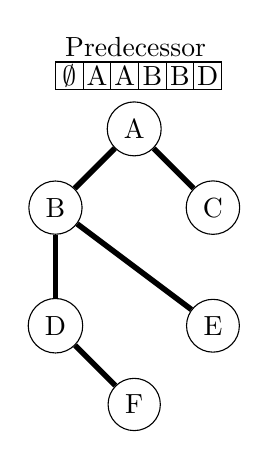
\begin{tikzpicture}
	\node [draw,circle] (node A) at (1,3.5) {A};
	\node [draw,circle] (node B) at (0,2.5) {B};
	\node [draw,circle] (node C) at (2,2.5) {C};
	\node [draw,circle] (node D) at (0,1) {D};
	\node [draw,circle] (node E) at (2,1) {E};
	\node [draw,circle] (node F) at (1,0) {F};
	
	\draw [line width=2pt] (node A) -- (node B);
	\draw [line width=2pt] (node A) -- (node C);
	\draw [line width=2pt] (node B) -- (node D);
	\draw [line width=2pt] (node B) -- (node E);
	\draw [line width=2pt] (node D) -- (node F);
	
	% The array under the graph
	%\foreach \x in{0,...,5}{\draw (\x*1em,-1) rectangle (\x*1em+1em,-1+1em);}
	\draw (0,4) rectangle (1em,4.35) node[pos=.5] {$\emptyset$};
	\draw (1em,4) rectangle (2em,4.35) node[pos=.5] {A}; % B
	\draw (2em,4) rectangle (3em,4.35) node[pos=.5] {A}; % C
	\draw (3em,4) rectangle (4em,4.35) node[pos=.5] {B}; % D
	\draw (4em,4) rectangle (5em,4.35) node[pos=.5] {B}; % E
	\draw (5em,4) rectangle (6em,4.35) node[pos=.5] {D}; % F

	\node [anchor=south west] at (0,4.3) {Predecessor};
\end{tikzpicture}
\caption{Example of Breadth First Search in an undirected graph}
\label{fig:part2_chap3:BFS}
\end{figure}


This algorithm is presented on figure~\ref{fig:part2_chap3:BFS}.
At each step from the current queue we search through the neighbors of nodes. 
All the new nodes, not yet traversed, are added in the queue for the next step.
We keep the information of neighbors exploration in order to recreate the predecessor array. 

This algorithm is very famous thanks to its use in many applications but also thanks to the world supercomputer ranking called Graph500\footnote{\url{http://www.graph500.org}}.
This benchmark is designed to measure the performance on very irregular problems like BFS on a large scale randomized generated graph. 
The first Graph500 list was released in November 2010.
The last list, issued in November 2017, is composed of 235 machines ranked using a specific metric: Traversed Edges Per Second, denoted as TEPS. 
The aim is to perform a succession of 64 BFS on a large scale graph in the fastest possible way.
Then the ratio of edges traversed per the time of computation is used to rank the machines.

This benchmark is more representative of communication and memory accesses than computation itself. 
Other benchmarks can be used to rank computational power such as LINPACK for the TOP500 list.
Indeed the best supercomputers (K-Computer, Sequoia, Mira, ...) on the ladder have a very specific communication topology and sufficient memory, and are large enough to quickly visit all the nodes of the graph. 

This benchmark is conduct using GPUs as accelerators.
There are many CPU algorithms available, which are listed on the Graph500 website. 
In order to rank the ROMEO supercomputer we had to create a dedicated version of the Graph500 benchmark in order to fit the supercomputer architecture. 
As this supercomputer is accelerated by GPUs, three successive approaches had to be applied:  first create an optimized CPU algorithm; second provide a GPU specific version and third take advantage of both CPU and GPU computation power. 

The first section performs a survey of graph representation and analysis; it also describes some specific implementations.
The second section  describes the Graph500 protocol and focuses on the Kronecker graph generation method and the BFS validation.
The third section presents the chosen methods to implement graph representation and work distribution over the supercomputer nodes. It particularly focuses on the interest of a hybrid CSR and CSC representation.
We compare the results for different graph scales and load distributions.

\section{Existing methods}
The most efficient algorithm to compute BFS traversal is used and detailed in \cite{6468459}. 
It uses a 2D partition of the graph which will be detailed later. 
This algorithm is used on the BlueGene/P and BlueGene/Q architectures but can be easily adapted to any parallel cluster.

We use another key study in order to build our Graph500 CPU/GPU implementation. 
\cite{merrill2015high} proposes various effective methods on GPU for BFS. 
Merrill \& al. explaine and teste a few efficient methods to optimize memory access and work sharing between threads on a large set of graphs. 
It focuses on Kronecker graphs in particular. 
First they propose several methods for neighbor-gathering with a serial code versus a warp-based and a CTA-based approach. 
They also use hybridization of these methods to reach the performance level. 
In a second part they describe the way to perform label-lookup, to check if a vertex is already visited or not. 
They propose to use a bitmap representation of the graph with texture memory on the GPU for fast random accesses. 
In the last phase, they propose methods to suppress duplicated vertices generated during the neighbor exploration phase. 
Then based on these operations they propose \textit{expand-contract}, \textit{contract-expand}, \textit{two-phase} and finally \textit{hybrid} algorithms to adapt the method with all the studied graph classes.
The last part they propose a multi-GPU implementation.
They use a 1D partition of the graph and each GPU works on its subset of vertices and edges. 

In \cite{fu2014parallel}, a first work is proposed to implement a multi-GPU cluster version of the Graph500 benchmark. 
The scheme used in their approach is quite similar to the one in our study but with a more powerful communication network, namely FDR InfiniBand. 

In our work we focus on the GPUDirect usage on the ROMEO supercomputer. 

\section{Environment}
As previously mentioned, a CPU implementation is available on the official Graph500 website. 
A large range of software technology is covered with MPI, OpenMP, etc. 
All these versions use the same generator and the same validation pattern which is described in this part below. 

The Graph500 benchmark is based on the following stages:
\begin{itemize}
	\item \textit{Graph generation.} The first step is to generate the Kronecker graph and mix the edges and vertices. 
	The graph size is chosen by the user (represented as a based-2 number of vertices). The $EDGEFACTOR$, average ratio of edges by vertex, is always $16$. 
	Self-loop and multiple edges are possible with Kronecker graphs.
	Then 64 vertices for the BFS are randomly chosen. 
	The only rule is that a chosen vertex must have at least one link with another vertex in the graph. \textit{This stage is not timed};
	\item \textit{Structure generation.} The specific code part begins here. 
	Based on the edge list and its structure the user is free to distribute the graph over the machines. 
	In a following section we describe our choices for the graph representation. \textit{This stage is timed};
	\item \textit{BFS iterations.} This is the key part of the ranking. Based on the graph representation, the user implements a specific optimized BFS. Starting with a root vertex the aim is to build the correct BFS tree (up to a race condition at every level), storing the result in a predecessor list for each vertex;
	\item \textit{BFS verification.} The user-computed BFS is validated. The number of traversed edges is determined during this stage.  
\end{itemize}

The process is fairly simple and sources can be found at \url{http://www.graph500.org}.
The real problem is to find an optimized way to use parallelism at several levels: node distribution, CPU and GPU distribution and then massive parallelism on accelerators.



\subsection{Generator}

The \textit{Kronecker graphs}, based on Kronecker products, represent a specific graph class
imposed by the Graph500 benchmark. 
These graphs represent realistic networks and are very useful in our case due to their irregular aspect~\cite{leskovec2010kronecker}. 
The main generation method uses the Kronecker matrix product. 
Based on an initiator adjacency matrix $K_1$, we can generate a Kronecker graph of order $K_1^{[k]}$ by multiplying $K_1$ by itself $k$ times. 
The Graph500 generator uses Stochastic Kronecker graphs, avoiding large scale matrix multiplying, to generate an edge list which is utterly mixed (vertex number and edge position) to avoid locality. 

\begin{figure}[!t]
	\centering
	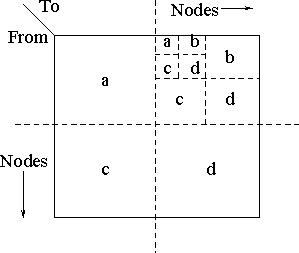
\includegraphics[scale=.9]{\locpath/figures/graph500/rmat_generation}
	\caption{Kronecker generation scheme based on edge probability}
	\label{fig:kron_gen_scheme}
\end{figure}

As presented on figure~\ref{fig:kron_gen_scheme}, the generation is based on edge presence probability on a part of the adjacency matrix. 
For the Graph500 the probabilities are $a = 0.57$, $b = c = 0.19$ and $d = 0.05$.
The generator handle can be stored in a file or directly split in the RAM memory of each process. 
The first option is not very efficient and imposes a lot of I/O for the generation and verification stage but can be very useful for large scale problems.
The second option is faster but uses a part of the RAM thus less ressources are available for the current BFS execution.


\subsection{Validation}
The validation stage is completed after the end of each BFS. 
The aim is to check if the tree is valid and if the edges are in the original graph.
 This is why we must keep a copy of the original graph in memory, file or RAM. 
This validation is based on the following stages, presented on the official Graph500 website.
First, the BFS tree is a tree and does not contain cycles.
Second, each tree edge connects vertices whose BFS levels differ by exactly one.
Third, every edge in the input list has vertices with levels that differ by at most one or that both are not in the BFS tree.
Finally, he BFS tree spans an entire connected component's vertices, and
a node and its parent are joined by an edge of the original graph.

In order to meet the Graph500 requirements we use the proposed verification function provided in the official code.

\section{BFS traversal}
In this section we present the actual algorithm we used to perform the BFS on a multi-GPU cluster. 
In a first part we introduce the data structure; then we present the algorithm and the optimizations used.

\subsection{Data structure}
We performed tests of several data structures.
In a first work we tried to work with bitmap. Indeed the regularity of computation can fit very well with the GPU architecture. But this representation imposes a significant limitation on the graph size. 
This representation is used on the BlueGene/Q architecture. 
Indeed they have some specific hardware bit-wise operations implemented in their processors and have a large amount of memory, allowing them to perform very large scale graph analysis. 

In a second time we used common graph representations, Compressed Sparse Row (CSR) and Compressed Sparse Column (CSC) representation, which fit very well with sparse graphs such as the Graph500 ones.

\begin{figure}[t!]
\begin{center}
\begin{tikzpicture}
\matrix[anchor=south east] at (0,-.8) (m) [matrix of nodes,nodes={rectangle,draw},
	row 1/.style={nodes={fill=black!20}},
	row 2/.style={nodes={fill=yellow!20}},
	row 3/.style={nodes={fill=cyan!20}},
	row 4/.style={nodes={fill=blue!20}}]
{
	0 & 1 & 1 & 0 \\ 
	1 & 0 & 1 & 0 \\ 
	1 & 1 & 0 & 1 \\ 
	0 & 0 & 1 & 0 \\    
};
\matrix[anchor=north west] at (1,1.5) (R) [matrix of nodes,nodes={rectangle,draw},
	column 1/.style={nodes={fill=black!20}},
	column 2/.style={nodes={fill=yellow!20}},
	column 3/.style={nodes={fill=cyan!20}},
	column 4/.style={nodes={fill=blue!20}}]
{
	0 & 2 & 4 & 7 &  8\\   
};
\node[anchor=east] at (R.west) {R =};
\matrix[anchor=north west] at (1,0) (C) [matrix of nodes,nodes={rectangle,draw},
	column 1/.style={nodes={fill=black!20}},
	column 2/.style={nodes={fill=black!20}},
	column 3/.style={nodes={fill=yellow!20}},
	column 4/.style={nodes={fill=yellow!20}},
	column 5/.style={nodes={fill=cyan!20}},
	column 6/.style={nodes={fill=cyan!20}},
	column 7/.style={nodes={fill=cyan!20}},
	column 8/.style={nodes={fill=blue!20}}]
{
	1 & 2 & 0 & 2 & 0 & 1 & 3 & 2 \\  
};
\node[anchor=east] at (C.west) {C =};
\draw[->] ([yshift=-2pt]R-1-1.south) -- ([yshift=2pt]C-1-1.north);
\draw[->] ([yshift=-2pt]R-1-2.south) -- ([yshift=2pt]C-1-3.north);
\draw[->] ([yshift=-2pt]R-1-3.south) -- ([yshift=2pt]C-1-5.north);
\draw[->] ([yshift=-2pt]R-1-4.south) -- ([yshift=2pt]C-1-8.north);
\end{tikzpicture}
\end{center}
\caption{Compressed Sparse Row example}
\label{fig:csr_representation}
\end{figure}

Figure~\ref{fig:csr_representation} is an example illustratinf the CSR compression.
The M adjacency matrix represents the graph. $R$ vector contains the cumulative number of neighbors for each vertex, of size $(\#vertices +1)$. $C$, of size $(\#edges)$, is, for each index of $R$, the edges of a vertex.
This representation is very compact and very efficient to work with sparse graphs. 

\subsection{General algorithm}

When looking at the latest Graph500 list we see that the best machines are the BlueGene ones. 
We count about 26 BlueGene/Q and BlueGene/P machines in the first 50  machines.
This is due to a quite specific version of the BFS algorithm proposed in \cite{6468459}. 
It proposes a very specific 2D distribution for parallelism and massive use of the 5D torus interconnect. 

In the BFS algorithm, like other graph algorithms, parallelism can take several shapes. 
We can split the vertices into partitions using 1D partition. 
Each thread/machine can then work on a subset of vertices. 
The main issue with this method is that the partitions are not equal since the number of edges per vertex can be very different; 
moreover in graphs like Kronecker ones where some vertices have a very high degree compared to other ones.
Thus we are confronted with a major load balancing problem. 

In \cite{6468459} they propose a new vision of graph traversal, here BFS, on distributed-memory machines. 
Instead of using standard 1D distribution their BFS is based on a 2D distribution. 
The adjacency matrix is split into blocks of same number of vertices.
If we consider $l\times l$ blocks $A_{i,j}$ we can split the matrix as follows:

\[ M = \left[ \begin{array}{cccc}
A_{0,0} & A_{0,1} & \cdots & A_{0,l-1} \\
A_{1,0} & A_{1,1} & \cdots & A_{1,l-1} \\
\vdots  & \vdots  & \ddots & \vdots    \\
A_{l-1,0} & A_{l-1,1}  & \cdots & A_{l-1,l-1} \end{array} \right] \] 

Each bloc $A_{x,y}$ is a subset of edges. 
We notice that blocks $A_{0,l-1}$ and $A_{l-1,0}$ have the same edges but in a reverse direction for undirected graphs. 
Based on this distribution they use \textit{virtual processors}, which are either machines or nodes, each associated with a block.
This has several advantages.
First we reduce the load balancing overhead and a communication pattern can be set up. 
Indeed each column shares the same $in\_queue$ and each row will generate an $out\_queue$ in the same range. 
Thus for all the exploration stages, communications are only on line and we just need a column communication phase to exchange the queues for the next BFS iteration.  
Algorithm~\ref{alg:bfs_bluegene} presents the BlueGene/Q and BlueGene/P parallel BFS.


\begin{algorithm}
\caption{Parallel BFS on BlueGene}\label{alg:bfs_bluegene}
\begin{algorithmic}[1]
\State $Vis_{i,j} \gets In_{i,j}$
\State $P(N_{i,j},v) \gets \bot$ \textbf{for all} $v \in R_{i,j}^{1D}$
\If{$v_s \in R_{i,j}^{1D}$}
\State $P(N_{i,j},v_s) \gets v_s$
\EndIf
\While{$true$}
	\State$(Out_{i,j},Marks_{i,j} \gets $ ExploreFrontier();
	\State $done \gets \bigwedge\limits_{0 \leq k, l \leq n} (Out_{k,l} = \emptyset)$
	\If{$done$}
		\State \textbf{exit loop}
	\EndIf
	\If{$j = 0$}
		\State $prefix_{i,j} = \emptyset$
	\Else 
		\State \textbf{receive} $prefix_{i,j}$ from $N_{i,j-1}$
	\EndIf
	\State $assigned_{i,j} \gets Out_{i,j} \setminus prefix_{i,j}$
	\If{$j \neq n -1$}
		\State \textbf{send} $prefix_{i,j} \cup Out_{i,j}$ \textbf{to} $N_{i,j+1}$
	\EndIf
	\State $Out_{i,j} \gets \bigcup\limits_{0 \leq k \leq n} Out_{i,k}$
	\State WritePred()
	\State $Vis_{i,j} \gets Vis_{i,j} \cup Out_{i,j}$
	\State $In_{i,j} \gets Out_{j,i}$
\EndWhile
\end{algorithmic}
\caption{Algorithm for tree traversal presented for BlueGene}
\label{alg:bluegene}
\end{algorithm}

This algorithm is presented in algorithm~\ref{alg:bluegene} and is based on the exploration phase, denoted by \textit{ExploreFrontier()}. It performs the exploration phase independently on all the machines.
Then several communication phases follow. 
The first two phases are performed on the same processes line. The last one is performed on a processes column. 
\begin{itemize}
	\item On line 15, an exclusive scan is performed for each process on the same line, all the $A_{i,x}$ with $i \in [0,l-1]$. 
	This operation allows us to know which vertices have been discovered in this iteration.
	\item On line  19, a broadcast of the current $out\_queue$ is sent to the processes on the same line. With this information they would be able to update the predecessor list only if they are the first parent of a vertex.
	\item On line 24, a global communication on each column is needed to prepare the next iteration. 
	The aim is to replace the previous $in\_queue$ by the newly computed $out\_queue$.
\end{itemize}

Two functions are not specified: 
\textit{ExploreFrontier()} converts the $in\_queue$ into $out\_queue$ taking account of the previously visited vertices;
\textit{WritePred()} aims to generate the BFS tree and therefore store the predecessor list. In this algorithm the predecessor distribution is still in 1D to avoid vertex duplication. 
	This part can be done using RDMA communication to update predecessor value or with traditional MPI all-to-all exchanges.
	It can be done during each iteration stage or at the end of the BFS but this requires using a part of the memory to store this data. 

This algorithm, which is the basis of many implementations, is the main structure of our distribution. 

\subsection{Direction optimization}

In order to get an optimized computation in terms of TEPS we decided to sacrifice a small part of the memory for storing both the CSC and CSR representations. 
Indeed during the different BFS iterations the $in\_queue$ size varies a lot and, taking this into account, it is wiser to perform exploration from \textit{top-down} or \textit{bottom-up}. 
So, as proposed in \cite{beamer2013direction}, we perform a direction-optimized BFS.

In the first case, \textit{top-down}, we start from the vertices in the $in\_queue$ and check all the neighbors verifying each time if this neighbor has ever been visited. 
Then if not, it is added to the $out\_queue$. 
When the $in\_queue$ is sparse, like for the first and latest iterations, this method is very efficient. 
In the second case, \textit{bottom-up}, we start the exploration by the not-yet-visited vertices and verify if there is a link between those vertices and the $in\_queue$ ones. 
If yes, the not-yet-visited vertex is added to the $out\_queue$. 
Table~\ref{table:direction_optimized} shows the advantages of swithing from top-dowm to bottom-up regarding the number of edges travered.
Figure~\ref{fig:csr_csc} presents the two approches, whith the time visiting all the edges, and the benefits of their hybridization.

\begin{table}[t!]
\centering
\begin{tabular}{c||r|r|r}
		%\hline 
		\textbf{Iteration} & \textbf{Top-down} & \textbf{Bottom-up} & \textbf{Hybridization} \\ 
		\hline 
		\hline 
		0 & \color{red}{27} & 22 090 111 & \color{red}{27} \\ 
		%\hline 
		1 & \color{red}{8 156} & 1 568 798 & \color{red}{8 156} \\ 
		\hline 
		2 & 3 695 684 & \color{blue}{587 893} & \color{blue}{587 893} \\ 
		%\hline 
		3 & 19 565 465 & \color{blue}{12 586} & \color{blue}{12 586} \\ 
		%\hline 
		4 & 214 578 & \color{blue}{8 256} & \color{blue}{8 256} \\ 
		%\hline 
		5 & 5 865 & \color{blue}{1 201} & \color{blue}{1 201} \\ 
		\hline 
		6 & \color{red}{12} & 156 & \color{red}{12} \\ 
		\hline
		\textbf{Total} & 23,489,787 & 24,269,001 & 618,131 
		%\hline 
\end{tabular} 
\caption{BFS directions change from top-down to bottom-up}	
\label{table:direction_optimized}
\end{table}

\begin{figure}[!t]
\begin{subfigure}[t]{.48\textwidth}
	\centering
	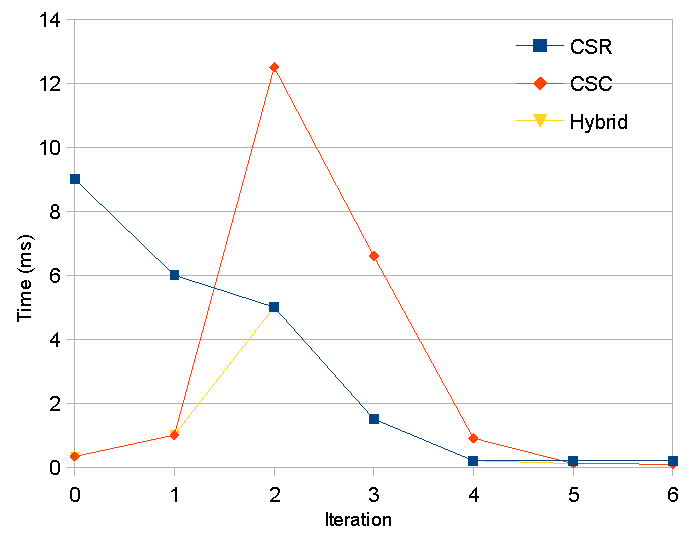
\includegraphics[width=1\columnwidth]{\locpath/figures/graph500/csr_csc_hybrid_iteration}
	\caption{CSR and CSC approach comparison. On a 6 iterations BFS, the time with the two method is compared. The hybridization just takes the best time of each method}
	\label{fig:csr_csc}
\end{subfigure}
\hfill
\begin{subfigure}[t]{.48\textwidth}
	\centering
	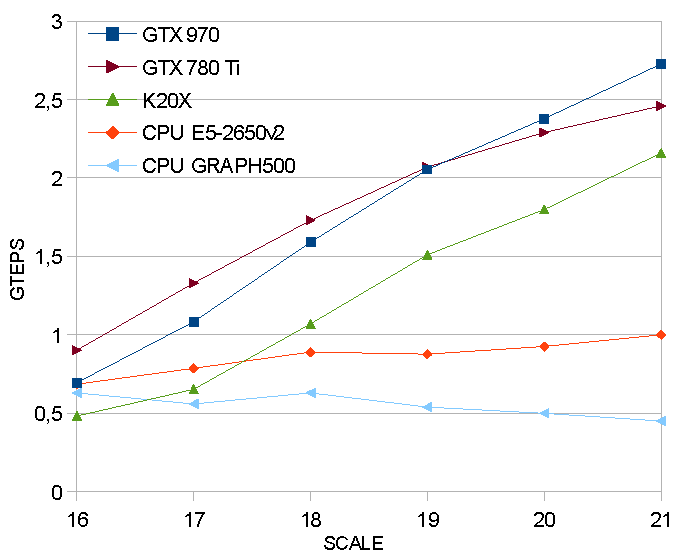
\includegraphics[width=1\columnwidth]{\locpath/figures/graph500/comparatif_GPU}
	\caption[]{Single CPU and accelerators comparison. CPU Graph500 represent the best implementation proposed by the Graph500 website. }
	\label{fig:single_cpu_accelerators}
\end{subfigure}
\end{figure}

\subsection{GPU optimization}

In algorithm~\ref{alg:bfs_bluegene}, two parts are not developed. namely \textit{ExploreFrontier()} and \textit{WritePred()}. Indeed these phases are optimized using the GPU. 
Based on the Merill et al. implementation, the algorithm is optimized to use the shared memory and the texture memory of the GPU. 
For our version we decided to keep the bitmap implementation for the communications and the queues. So we have to fit the CSR and CSC implementations. 
On algorithm~\ref{alg:csr} we present the CSR algorithm;
CSC is based on the same approach but starting from the $visited$ queue. 

In the CSR version each warp is attached to a 32 bit word of the $in\_queue$ bitmap. 
Then if this word is empty the whole warp is released; 
if it contains some vertices, the threads collaborate to load the entire neighbor list. 
Then they access the coalescent area in the main memory to load the neighbor list. 
A texture memory is used to accelerate the verification concerning this vertex. Indeed this memory is optimized to be randomly accessed. 
Then the vertex is added in the bitmap $out\_queue$.

\begin{algorithm}
\caption{Exploration kernel based on CSR}\label{alg:csr}
\begin{algorithmic}[1]
\State \textbf{Constants:}
\State $NWARP$: number of WARPS per block
\State 
\State \textbf{Variables:}
\State $pos\_word$: position of the word in $in\_queue$
\State $word$: value of the word in $in\_queue$
\State $lane\_id$: thread ID in the WARP
\State $warp\_id$: WARP number if this block
\State $comm[NWARP][3]$: shared memory array
\State $shared\_vertex[NWARP]$: vertex in shared memory
\State 
\State \textbf{Begin}
\If{$word = 0$}
\State free this WARP
\EndIf
\If{$word\ \& 1\ << lane\_id$}
\State $id\_sommet \gets = pos\_word*32+lane\_id$
\State $range[0] \gets C[id\_sommet]$ 
\State $range[1] \gets C[id\_sommet +1 ]$ 
\State $range[2] \gets range[1] - range[0]$ 
\EndIf
\While{$\_\_any(range[2])$}
\If{$range[2]$}
\State $comm[warp\_id][0] \gets lane\_id$
\EndIf
\If{$comm[warp\_id][0] \gets lane\_id$}
\State $comm[warp\_id][0] \gets range[0]$
\State $comm[warp\_id][0] \gets range[1]$
\State $range[2] \gets 0$
\State $share\_vertex[warp\_id] = id\_sommet$ 
\EndIf

\State $r\_gather \gets comm[warp\_id][0] + lane\_id$
\State $r\_gather\_end \gets comm[warp\_id][2] $
\While{$r\_gather < r\_gather\_end$}
	\State $voisin \gets R[r\_gather]$
	\If{$not \in tex\_visited$}
		\State Adding in $tex\_visited$
		\State AtomicOr($out\_queue$,$voisin$)
	\EndIf
	\State $r\_gather \gets r\_gather + 32$
\EndWhile
\EndWhile
\end{algorithmic}
\end{algorithm}

 
\subsection{Communications}

Based on the algorithm \ref{alg:bfs_bluegene} communications pattern, we first used MPI with the CPU transferring the data. But the host-device transfer time between the CPU and the GPU was too time-consuming. 
In order to accelerate the transfers between the GPUs, we used a specific GPU MPI-aware  library. This library allows direct MPI operations from the memory of one GPU to another and also implements direct GPU collective operations. 
GPUDirect can be used coupled with this library. In the last version we used this optimization with GDRCopy. 

\section{Results}

\subsection{CPU and GPU comparison}

On figure~\ref{fig:single_cpu_accelerators} we present the single node implementation. 
Here we compare the best CPU implementation proposed by the Graph500 benchmark with our GPU implementation. 
On our cluster we worked with K20Xm GPUs. 
The GPU result is twice times better than the CPU one. 
We also carried out tests on some "general public" GPUs like GTX980 and GTX780Ti. 
The result is better on these GPUs because they do not implement the ECC memory and do not provide double precision CUDA cores. 
Indeed all the cores can be used for the Exploration phase. 



\subsection{Strong and weak scaling}

On figure~\ref{fig:bfs_strong_scaling} and figure~\ref{fig:bfs_weak_scaling} we see the result of strong and weak scaling. 
In the strong scaling we used a $SCALE$ of $21$ for different numbers of GPUs. 
The application scales up to 16 GPUs but then the data exchanges are too penalizing;
performance for 64 GPUs is lower. 
Indeed as the problem scale does not change, the computational part is reduced compared to the communication one. 
Using 16 GPUs we were able to perform up to 4.80 GTEPS. 


For the weak scaling, the $SCALE$ evolves with the number of GPUs. 
So the computation part grows and the limitation of communications is reduced. 
On figure~\ref{fig:bfs_weak_scaling}, the problem SCALE is presented on each point. 
With our method we were able to reach up to 12 GTEPS using this scaling. 


\subsection{Communications and GPUDirect}

Each node of the ROMEO supercomputer is composed of two CPU sockets and two GPUs, named GPU 0 and GPU 1.
Yet the node just has one HCA (Host Channel Adapters), linked with CPU 0 and GPU 0. 
In order to use this link GPU 1 has to pass through a Quick Path Interconnect link (QPI) between the two CPU sockets. 
This link considerably reduces the bandwidth available for node-to-node communication. 
Another problem is that the two GPUs have to share the same HCA for their communication. 


\begin{figure}[htb]
\begin{subfigure}[t]{0.48\linewidth}
\centering
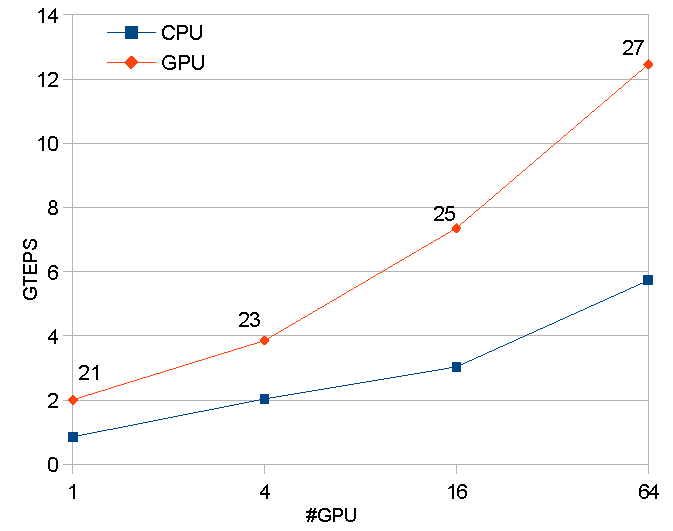
\includegraphics[width=1\linewidth]{\locpath/figures/graph500/weak_scaling}
\caption[]{CPU \textit{vs} GPU weak scaling. The number of CPUs is the same as the number of GPUs.}
\label{fig:bfs_weak_scaling}
\end{subfigure}
\hfill
\begin{subfigure}[t]{0.48\linewidth}
\centering
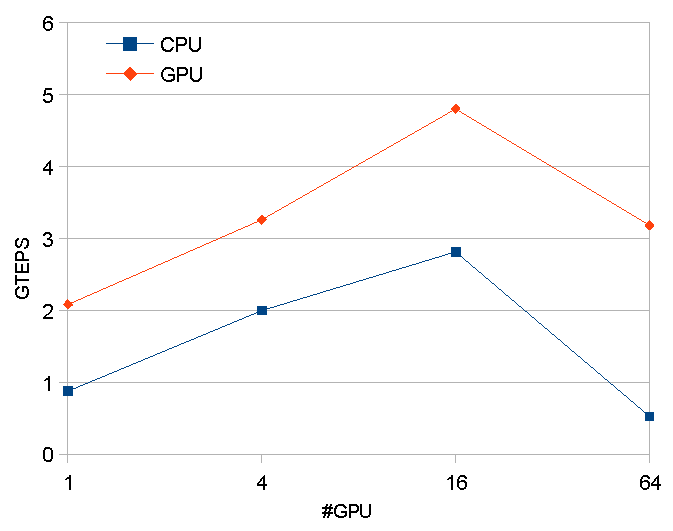
\includegraphics[width=1\linewidth]{\locpath/figures/graph500/strong_scaling}
\caption[]{CPU \textit{vs} GPU strong scaling. The $SCALE$ is showed on the GPU line. The number of CPUs is the same as the number of GPUs.}
\label{fig:bfs_strong_scaling}
\end{subfigure}
\caption{Weak and Strong scaling between CPU and GPU}
\end{figure}


On figure~\ref{fig:full_vs_gpu0}, the tests are based on the GPU-only implementation. 
First we worked with the two GPUs of the nodes. 
We were able to perform up to to $SCALE$ 29 with 12 GTEPS. 
The GPUDirect implementation does not allow the communication with a QPI link. 
So in order to compare the results, we used only the GPU 0 of each node of the supercomputer. 
Based on our algorithm implementation we need to use a number $2^{2n}$ of GPUs. 
Then the tests on figure~\ref{fig:full_vs_gpu0} are for 256 GPUs (with GPU 0 and GPU 1) and with 64 GPUs (using just GPU 0 only). 
Thus we were able to reach a better value of GTEPS. 
As the major limitation is the communications stage, using only GPU 0 allowed us to obtain about 13.70 GTEPS on the ROMEO supercomputer. 

\begin{figure}[!t]
\centering
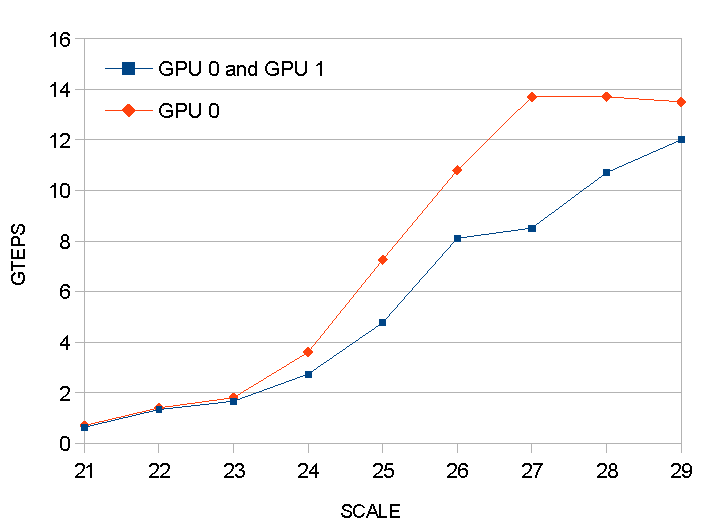
\includegraphics[width=.5\columnwidth]{\locpath/figures/graph500/full_vs_gpu0}
\caption[]{Full node GPUs \textit{vs} GPU 0. The GPU 0 implementation not use the QPI link of the two CPU socket.}
\label{fig:full_vs_gpu0}
\end{figure}

\section{Conclusions}
%\todo{Repenser la conclusion}

The Graph500 is already a benchmark and focus on memory and communication wall in an irregular behavior.
We presented an optimized implementation of the Graph500 benchmark for the ROMEO  multi-GPU cluster for the purpose of our metric to emphasis behavior of hybrid architectures.
It is based on the BlueGene/Q algorithm and GPU optimization for BFS traversal by Merrill et al. 
This work highlights different key points.
First, we have chosen a hybrid memory representation of graphs using both CSR and CSC. % data representation. 
Although this representation requires more memory, it significantly reduces  the computation workload and allows us to achieve outstanding performance.
Second, the inter-node and intra-node communication is a critical bottleneck. 
Each compute node has two GPUs, however only one shares the same PCIe bridge with the Infiniband HCA that allows to take advantage of the GPUDirect technology.
Third, due to the low compute power needed for BFS traversal, we get better performance by fully loading GPUs.
Otherwise communication time cannot be overlapped with computation time. 
Thus to achieve the best performance we had to use only half of each node.
Finally, using all these optimizations, we achieved satisfactory results. 
Indeed, by using GPUDirect on 64 GPUs,  we are able to achieve 13,70 GTEPS. 
In this configuration CPUs are only used to synchronize GPUs kernels. 
All the communications are directly GPU to GPU using a CUDA-aware MPI library and GPUDirect.

These results have been published in the Graph500 list of November 2016 list. 
The ROMEO supercomputer was ranked 105th.\\ 

In addition to the previous benchmarks proposed in our thesis, the Graph500 complete the communication and memory irregular behavior. 
It shows the benefit of using many-core architectures in this context allowing twice better results using accelerators than CPUs.
 